\subsection{Система считывания и сбора данных эксперимента CBM}\label{sec:CBMreadout}

% Концентрация и ввод данных в ЭВМ (из статьи) смёрджено
Блок-схема архитектуры системы считывания и сбора данных эксперимента CBM приведена на \figref{fig:CBMreadout}.
В концепции системы сбора данных эксперимента CBM предусмотрено 4~функциональных уровня, каждый из которых реализован соответствующими платами. В общем случае к детектору примыкает плата передней электроники (FEB --- front-end board), где осуществляются аналоговые преобразования и оцифровка сигналов.
В зависимости от технологии детектора и требований к его характеристикам обработка сигнала должна осуществлятся разными способами. Следовательно для каждого детектора выбирается соответствующий чип для FEB.
Далее, данные в виде электрических цифровых сигналов поступают в контроллер считывания (ROC --- read-out controller), где происходит концентрация данных и их пересылка по оптическому каналу. На следующем уровне расположены платы обработки данных (DCB --- data combiner board). DCB уплотняют данные с различных детекторов за счет удаления избыточной информации специфическим для каждого детектора способом и группируют эти данные в пакеты, называемые срезами времени (time slice). В каждый срез времени попадают сообщения со всех детекторов, имеющие временную отметку в заданном интервале. Далее они передаются по меньшему числу оптических каналов с более высокой пропускной способностью~\cite{DPB}. После этого данные поступают в память, доступную центральному процессору ЭВМ по высокоскоростной шине через платы интерфейса, называемые FLIB.
%Аббревиатура FLIB обозначает FLES Interface Board, а FLES~\cite{FLES}, в свою очередь, обозначает First Level Event Selector, т.е. специализированный аппаратно-программный комплекс для построения событий ``на лету'' и их отбора по заданным критериям. Плата FLIB может быть реализована, например, путем программирования коммерческой PCI-E платы HTG~K-7.

\todo раскомментировать?

\begin{figure}[H]
\centering
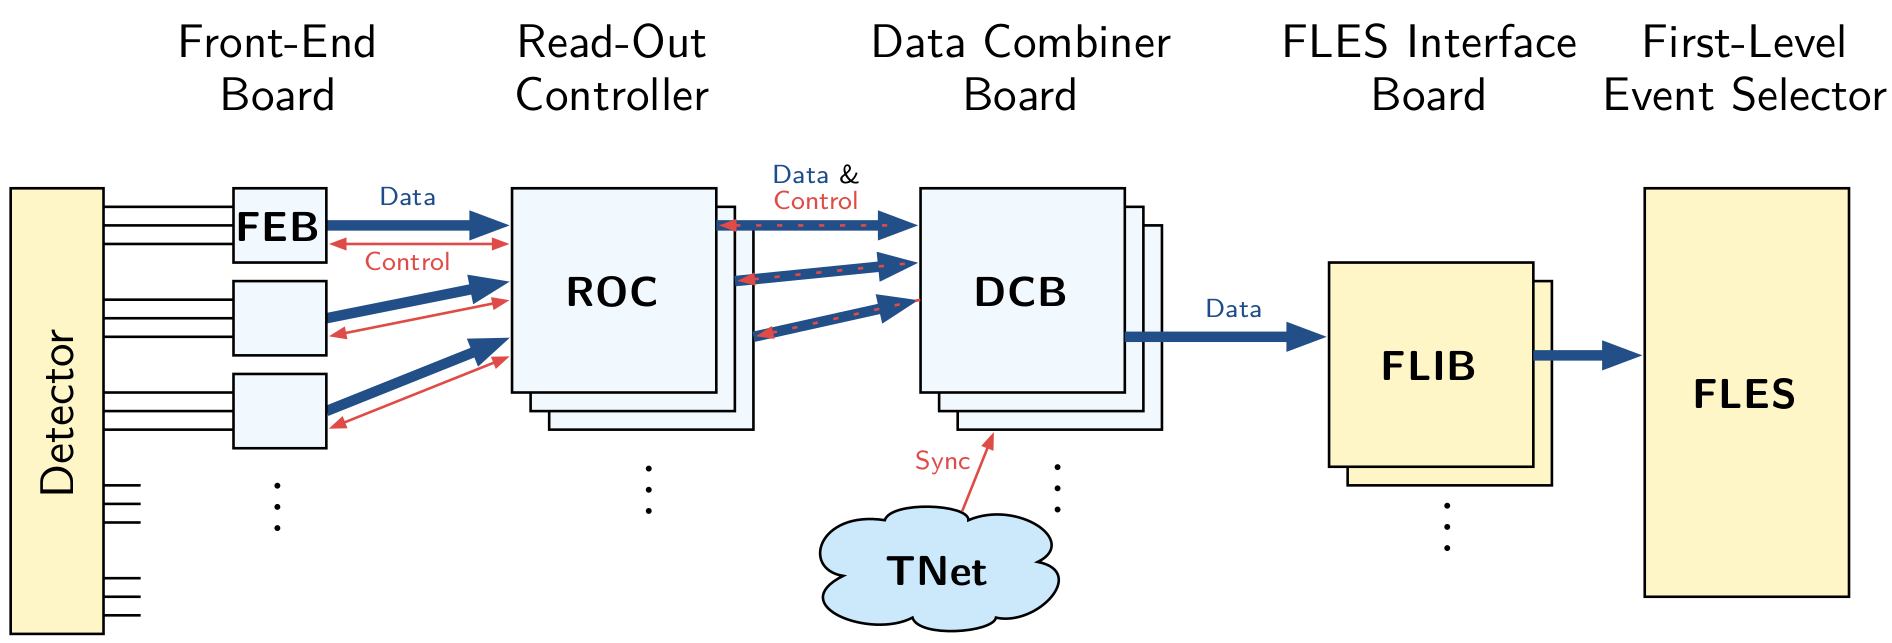
\includegraphics[width=0.7\textwidth]{pictures/CBMreadout.png}
\caption{Система считывания и сбора данных CBM.}
\label{fig:CBMreadout}
\end{figure}

\subsubsection{Система отбора первого уровня FLES}\label{sec:secFLES}

% ----------------------------------------------------------------------------------------------
% поиск хитов и трекинг в STS, 4d реконструкция
\bigskip
% ----------------------------------------------------------------------------------------------

FLES (First Level Event Selector) --- аппаратно-программный комплекс для отбора событий первого уровня. По сути DAQ-часть (приём данных) неотделима от FLES, поэтому иногда эту систему называют FLES/DAQ.
Отличительные черты FLES --- самотриггирующаяся электроника, несколько уровней концентрации данных, многочисленные буферы, формирование срезов времени, построение интервалов и только после этого --- построение событий.

% 1 - Приём данных и формирование срезов времени
Функционал FLES/DAQ можно разбить на три части. Первая --- приём и объединение данных, поступающих с группы каналов, в срезы времени (timeslice). Такую группу образует некоторое множество каналов одного детектора, количество которых определяется ожидаемым потоком данных, а ограничение диктуется максимальной пропускной способностью входного канала FLES.

% 2- Interval building
Один из наиболее важных и нестандартных этапов работы FLES --- это построение интервалов (Interval building, IB). Построение интервалов --- это получение контейнеров с данными со всех детекторов за некоторый интервал времени путём перегруппировки данных из срезов времени. Суть построения интервалов показана на \figref{fig:IntervalBuilding}. Данные от одного ``входного узла'' (input node, IN) приходят от группы каналов какого-то детектора и представляет собой последовательность срезов времени. Задача заключается в том, чтобы объединить все срезы, соответствующие одному интервалу времени, чтобы дальше передать на ``вычислительный узел'' (processing node, computing node, CN).

\begin{figure}[H]
\centering
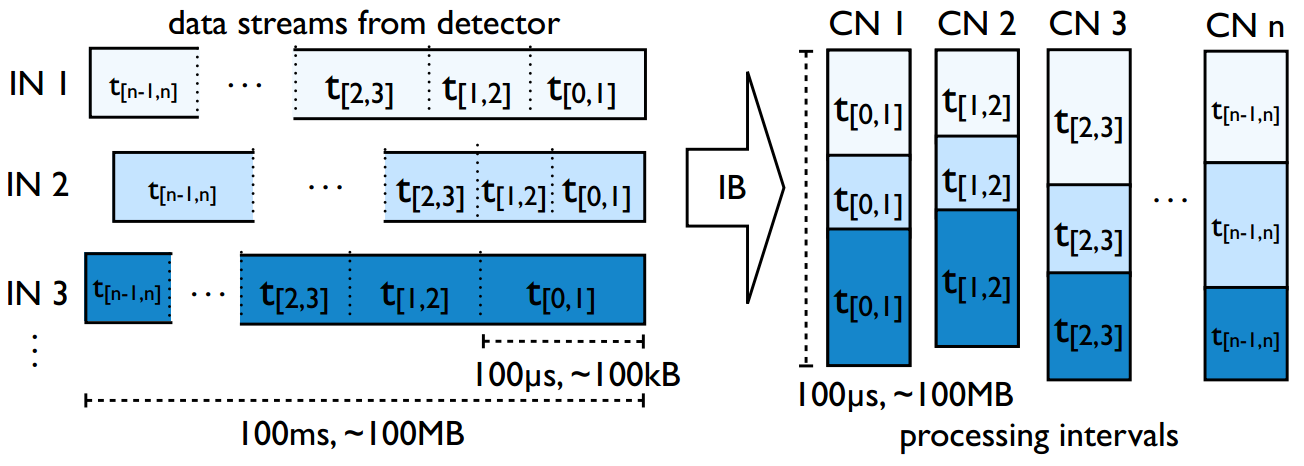
\includegraphics[width=0.7\textwidth]{pictures/Interval_building.png}
\caption{Построение интервала.}
\label{fig:IntervalBuilding}
\end{figure}

% 3- Этап после построения интервалов
Заключительный этап обработки данных во FLES --- восстановление событий в интервале, реконструкция треков и частиц в восстановленных событиях и выработка сигнала о сохранении или отбросе интервала.

%\subsubsection{Построение события}
Для выполнения реконструкции частиц для дальнейшего физического анализа необходимо сгруппировать треки, соответствующие одному событию. Эту задачу решает процедура простроения события.
Если частота первичных взаимодействий невысокая, то между отдельными событиями имеются достаточно длительные интервалы времени, позволяющие разделять сигналы исключительно по временной информации. Такой подход рассматривается в CBM как один из вариантов, но его применимость, очевидо, ограничена частотой первичных взаимодействий.
Эксперименты с высокой частотой имеют такую особенность, что события могут перекрываться во времени. В этом случае временная отметка хита может использоваться как четвёртая координата в алгоритмах поиска треков.
В частности в алгоритме поиска треков, используемом в CBM и основанном на клеточном автомате (\cite{}), время используется как 4-я координата при построении сегментов и при фитировании трека с помощью Фильтра Кальмана (\cite{}).
%\subsubsection{Введение 4-й координаты в трекинг}
В классическом варианте построение сегментов выполняется исключительно по координатам, а в 4d-трекинге помимо геометрических координат рассматривается и временная координата $(x, y, z, t)$. Если обычно для образования сегмента хит на следующей станции должен находиться в пределах заданного телесного угла, то теперь он также должен находиться в заданном интервале по времени.
В процедуре фитирования треков, которая выполняется в CBM STS с помощью фильтра Кальмана, выполняется расширение вектора состояния на временную координату $(x, y, t_{x}, t_{y}, q/p, t)$.

% Численные оценки, определение FLES как сети из узлов
Для эксперимента CBM был выполнен оценочный расчёт. Отправная точка --- возможно сохранение 1~Гбайт/сек данных. Считается, что одно событие CBM в среднем имеет объём 40~Кбайт. Отсюда следует, что максимальная частота первичного взаимодействия может быть 25~кГц. В стартовой конфигурации CBM частота первичного взаимодействия равна 10~МГц, следовательно, необходимо уменьшить поток данных в 400~раз. В полноценном режиме работы CBM ожидается 25~МГц, т.е. $ 25 \cdot 10^{6} \cdot 40 $ Кбайт = 1 Тбайт/сек. Планируется разбить этот поток в 1~Тбайт/сек на 1000 входных каналов FLES, каждый по 1~Гбайт/сек, передающихся по 10-Гбитным оптическим каналам связи. Один входной канал FLES соответствует одному ``входному узлу'' --- ЭВМ с установленной платой FLIB. Все вычисления, необходимые для отбора данных будут осуществляться на так называемых ``вычислительных узлах''. Входные и вычислительные узлы объединены в компьютерную сеть посредством InfiniBand QDR, образуя уникальную распределённую вычислительную систему, называемую FLES, см. \figref{fig:FLESarch}. Вычислительная подсеть будет иметь приблизительно 60000 ядер.

\begin{figure}[H]
\centering
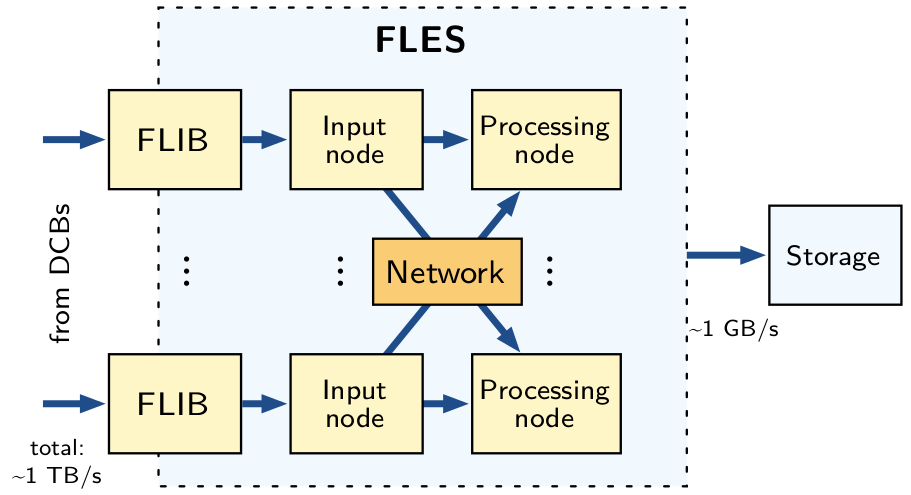
\includegraphics[width=0.7\textwidth]{pictures/FLESarch.png}
\caption{Общая схема устройства FLES.}
\label{fig:FLESarch}
\end{figure}

% Реконструкция по одному детектору
%Планируется также, что FLES сможет функционировать в особом режиме, когда для выполнения реконструкции с целью отбора данных для сохранения будет использоваться только часть входного потока. Это имеет смысл при работе эксперимента над некоторыми пунктами физической программы, но принципиальная возможность и эффективность реконструкции частиц с целью триггирования по ограниченному набору детекторов является предметом исследований. Например, можно восстанавливать \todo такую-то частицу только по трекам в MUCH. При этом система приёма данных работает в полную силу --- идёт приём со всех детекторов и никакие данные не выбрасываются до тех пор, пока не будет выполнена реконструкция по данным с MUCH. Если в результате реконструкции выясняется, что принятая порция данных потенциально интересна, то она извлекается из буферов и записывается. Это позволяет \todo снизить поток сохраняемых данных в \todo раз, что особенно актуально при экстремально высоких частотах взаимодействия.

%На \figref{fig:PartialIB} приведена блок-схема функционирования FLES в таком режиме. Синим блоком слева обозначены детекторы, которые используются для трекинга с целью отбора, залёным --- остальные. Синими стрелками обозначены потоки данных от детекторов, используемых для отбора. Данные от них поступают через входные узлы (input nodes) и коммутацию в вычислительные узлы (processing nodes), где выполняется частичное построение интервалов, реконструкция и выбор под-интервала. Затем идёт запрос остальных данных выбранного под-интервала (красные стрелки), которые поступают в буфер вычислительной сети (зелёные стрелки) вместе с изначально выбранными данными. Там выполняется полная реконструкция и запись данных в хранилище.

%\begin{figure}[H]
%\centering
%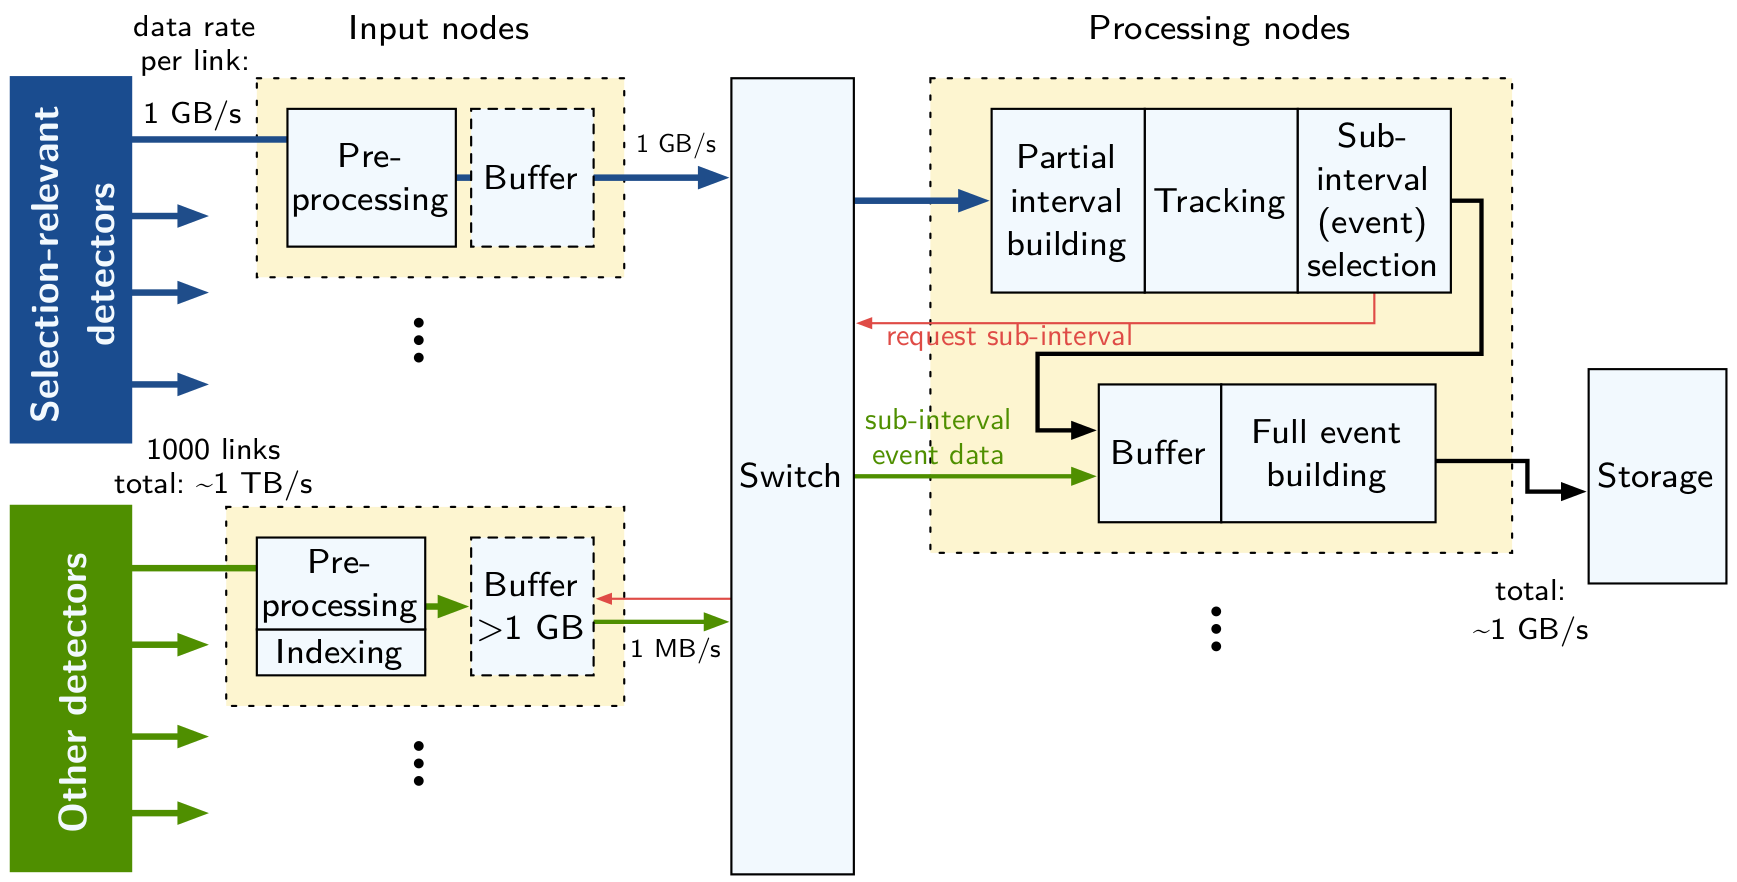
\includegraphics[width=1.0\textwidth]{pictures/PartialIB.png}
%\caption{Блок-схема функционирования FLES в режиме отбора по данным с части детекторов.}
%\label{fig:PartialIB}
%\end{figure}

%\todo найти use-case --- MUCH
